\documentclass[11pt]{amsart}

\usepackage[utf8]{inputenc}
\usepackage[T1]{fontenc}
\usepackage{amsmath,amssymb,amsthm}
\usepackage{graphicx}
\usepackage{booktabs}
\usepackage{array}
\usepackage{url}
\usepackage[hidelinks]{hyperref}
% \usepackage{microtype} % requires scalable fonts
\usepackage{geometry}
\geometry{margin=1in}

\newtheorem{theorem}{Theorem}
\newtheorem{result}[theorem]{Computational Result}
\theoremstyle{remark}
\newtheorem{remark}[theorem]{Remark}

\newcommand{\Z}{\mathbb{Z}}
\newcommand{\Q}{\mathbb{Q}}
\newcommand{\R}{\mathbb{R}}
\newcommand{\norm}[1]{\lVert #1 \rVert}

\title{Computational Bounds on Polynomial Relations\\
Among Fundamental Transcendental Constants:\\
Bivariate, Trivariate, and Statistical Evidence}

\author{M.~Narcisi}
\address{Independent researcher, Italy}

\subjclass[2020]{11Y60 (primary), 11J85, 11J91, 62G10 (secondary)}

\keywords{PSLQ algorithm, integer relations, algebraic independence,
transcendental constants, bivariate polynomials, computational number theory}

\begin{document}

\begin{abstract}
We present the most extensive computational search for
polynomial relations among fundamental transcendental
constants. Using PSLQ with precision up to 5{,}166 decimal
digits, we search for bivariate relations
$P(\alpha,\beta)=0$ among 19~pairs drawn from
$\{\pi,e,\gamma,\zeta(3),G,\Omega,\zeta(5),A,\ln 2\}$,
establishing exclusion bounds up to degree~40.
We extend to 10~trivariate triples (degrees up to~6),
extract near-miss diagnostics, and compare residuals
against 200~pseudo-generic baseline pairs via KS, AD, and
MW tests. No relation is found. The residual behavior is
statistically indistinguishable from generic constants
($p>0.25$; Cohen's $d=0.08$), supporting algebraic
independence. Each bound connects to open conjectures
including Schanuel's conjecture. The computation comprised
2{,}571 PSLQ runs over ${\approx}\,24$~hours wall-clock
on a 12-core workstation.
\end{abstract}

\maketitle

%% ====================================================================
\section{Introduction}\label{sec:intro}
%% ====================================================================

\subsection{Background and motivation}\label{ssec:background}

The algebraic independence of fundamental mathematical constants is among the deepest
open problems in transcendence theory. While individual transcendence results are
classical---Hermite (1873) for~$e$, Lindemann (1882) for~$\pi$, Ap\'ery (1978) for
the irrationality of~$\zeta(3)$---the question of whether two given transcendental
constants satisfy a polynomial relation with integer coefficients remains wide open
in most cases.

The strongest known theoretical result in this direction is Nesterenko's theorem
(1996)~\cite{Nesterenko1996}, which establishes the algebraic independence of the
triple $\{\pi, e^\pi, \Gamma(1/4)\}$ over~$\Q$. However, the algebraic independence
of even the most basic pair $(\pi,e)$ remains unproven, and is implied only by the
far-reaching Schanuel conjecture~\cite{Lang1966}.

In the absence of theoretical proofs, computational searches using integer relation
algorithms provide rigorous \emph{negative} evidence: when the PSLQ
algorithm~\cite{FergusonBailey1991,FergusonBaileyArno1999} terminates normally
without finding a relation, it certifies a lower bound on the Euclidean norm of any
integer relation vector that might exist. This approach was pioneered by
Bailey~\cite{Bailey1988,BaileyBorwein2013} and Bailey \&
Ferguson~\cite{BaileyFerguson1989}, who used early integer relation algorithms to
establish that certain constants do not satisfy low-degree univariate polynomial
equations with small coefficients.

\subsection{Prior computational work}\label{ssec:prior}

The computational literature on integer relations among constants can be organized
into several categories.

\medskip\noindent\textbf{(a) Univariate algebraicity tests.}
Bailey~\cite{Bailey1988} (1988) and Bailey \& Ferguson~\cite{BaileyFerguson1989}
(1989) tested whether individual constants ($\gamma$, $\log\gamma$, $\log\pi$,
$\zeta(3)$, $G$, etc.)\ satisfy univariate integer polynomials, establishing norm
bounds at various degrees. For example, Bailey \& Ferguson established that if
$\gamma$ satisfies an integer polynomial of degree~$\le 50$, then the Euclidean norm
of its coefficient vector must be very large. These results provide evidence that the
individual constants are transcendental (which is proven for $\pi$ and~$e$, but
remains open for $\gamma$, $\zeta(3)$, $G$, and others).

\medskip\noindent\textbf{(b) Linear integer relations.}
Bailey \& Ferguson~\cite{BaileyFerguson1989} (1989) searched for linear relations of
the form $a_1\alpha_1 + a_2\alpha_2 + \cdots + a_n\alpha_n = 0$ among sets of
constants, with the vector dimension~$n$ corresponding to the number of terms. They
established that certain sets of constants do not satisfy any such relation with
coefficient norm below specified bounds.

\medskip\noindent\textbf{(c) Discovery of specific identities.}
The PSLQ algorithm has been spectacularly successful in \emph{discovering} new
formulas, including the BBP formula for~$\pi$~\cite{BaileyBorweinPlouffe1997}, Euler
sum identities~\cite{BaileyBorweinGirgensohn1994}, and polylogarithmic
constants~\cite{BaileyBroadhurst2001}. The Ramanujan Machine
project~\cite{Raayoni2021,Elimelech2024} has recently automated the discovery of
continued fraction representations.

\medskip\noindent\textbf{(d) Bivariate polynomial relations.}
To the best of our knowledge, no prior published work has reported explicit degree
bounds for bivariate polynomial relations $P(\alpha,\beta)=0$ between specific pairs
of transcendental constants at degrees beyond approximately~$8$--$10$, although the
Ramanujan Library project~\cite{Elimelech2024} has explored polynomial relations
among constants in a broader automated discovery framework. This is the gap that the
present work addresses.

\subsection{Contribution}\label{ssec:contribution}

We conduct a systematic high-degree search for bivariate polynomial relations among
transcendental constants, pushing to total degree~40 for the top-priority pairs. The
key methodological approach enabling this is the use of dynamically scaled precision
following the Bailey precision criterion (Section~\ref{ssec:precision}), which
ensures that the PSLQ algorithm operates with sufficient arithmetic precision for
each (degree, coefficient-bound) combination.

Our results establish that for each of the 19~pairs tested, no non-trivial bivariate
polynomial relation exists within the searched parameter space. We emphasize that
these are \emph{rigorous computational bounds}, not heuristic estimates: they follow
from the proven termination and correctness properties of the PSLQ
algorithm~\cite{FergusonBaileyArno1999}.

Beyond the bivariate exclusion bounds, we make five additional contributions:
\begin{enumerate}
\item \textbf{Near-miss analysis} (Section~\ref{ssec:nearmiss}): We extract
  PSLQ's best candidate vectors from the internal $B$-matrix and quantify the
  \emph{precision fraction} $\lambda = -\log_{10}|R|/p$, confirming that no
  anomalous cancellation occurs across 138~vectors at degrees 3--12.
\item \textbf{Trivariate extension} (Section~\ref{sec:trivariate}): We search
  for $P(\alpha,\beta,\gamma)=0$ among 10~constant triples at degrees up to~6,
  establishing what we believe are the first systematic trivariate exclusion bounds.
\item \textbf{Statistical analysis} (Section~\ref{sec:statistics}): We compare
  the residual distributions of the real constants against a null model of 30
  pseudo-generic transcendental pairs using formal hypothesis tests.
\item \textbf{Exclusion frontiers}: We visualize the boundary in the (degree,
  coefficient norm) plane beyond which PSLQ can no longer certify non-existence.
\item \textbf{Conjecture connections}: We map each exclusion bound to specific
  open conjectures in transcendence theory.
\end{enumerate}

\subsection{Scope and limitations}\label{ssec:scope}

We state clearly what our results do and do not establish.

\begin{itemize}
\item \textbf{What we prove (computationally):} For each pair $(\alpha,\beta)$ and
  each tested $(d,M)$, there is no polynomial $P\in\Z[x,y]$ with $\deg(P)\le d$ and
  $\norm{c}_\infty\le M$ such that $P(\alpha,\beta)=0$. This is a rigorous
  consequence of PSLQ's termination properties.

\item \textbf{What we do not prove:} We do not prove algebraic independence. A
  relation with coefficients exceeding our bounds, or of degree exceeding our
  maximum, could still exist. Our results provide \emph{computational evidence}
  supporting the conjecture of algebraic independence, but they are not a proof.

\item \textbf{Implementation caveat:} Our bounds rely on the correctness of the
  \texttt{mpmath}~\cite{mpmath} implementation of PSLQ. While \texttt{mpmath} is a
  widely used and well-tested library, it is not a formally verified implementation.
  The rigorous bound guarantee of Ferguson--Bailey--Arno~\cite{FergusonBaileyArno1999}
  applies to the theoretical PSLQ algorithm; our results inherit the numerical
  reliability of \texttt{mpmath}'s implementation. We mitigate this by using a safety
  factor of $s=2.0$ on precision (twice the theoretical minimum) and by setting
  \texttt{maxsteps} to $10^7$ (the default limit of~100 is insufficient for
  high-degree searches), ensuring the algorithm runs to full convergence rather
  than terminating early. Additionally, all constant values are
  computed using \texttt{mpmath} with \texttt{gmpy2} backend, which provides
  arbitrary-precision arithmetic based on the GMP library.
\end{itemize}

%% ====================================================================
\section{Theoretical Framework}\label{sec:theory}
%% ====================================================================

\subsection{Problem formulation}\label{ssec:formulation}

Given a pair of real constants $(\alpha,\beta)$, we seek integer coefficients
$c_{ij}$ such that
\begin{equation}\label{eq:poly}
  P(\alpha,\beta) = \sum_{i+j\le d} c_{ij}\,\alpha^i\,\beta^j = 0,
\end{equation}
where $d$ is the total degree and $c_{ij}\in\Z$ with not all $c_{ij}=0$.

This is equivalent to finding an integer relation among the
$N(d) = \binom{d+2}{2} = (d+1)(d+2)/2$ real numbers
\begin{equation}\label{eq:monvec}
  \mathbf{v} = (1,\;\alpha,\;\beta,\;\alpha^2,\;\alpha\beta,\;\beta^2,\;\ldots,\;\beta^d),
\end{equation}
i.e., an integer vector $\mathbf{m}\in\Z^{N(d)}$ such that
$\mathbf{m}\cdot\mathbf{v}=0$.

\subsection{The PSLQ algorithm}\label{ssec:pslq}

We use the PSLQ integer relation algorithm of Ferguson and
Bailey~\cite{FergusonBailey1991,FergusonBaileyArno1999}. Given a real vector
$\mathbf{x}=(x_1,\ldots,x_n)$ and a working precision of~$p$ decimal digits, PSLQ
either:
\begin{enumerate}
\item \textbf{Finds} an integer vector $\mathbf{m}$ with
  $\mathbf{m}\cdot\mathbf{x}=0$ (within precision), or
\item \textbf{Certifies} that no such vector exists with $\norm{\mathbf{m}}<B$,
  where $B$ is a bound derived from the algorithm's internal $H$~matrix.
\end{enumerate}

Property~(2) is the source of our negative bounds. Specifically, if PSLQ terminates
without finding a relation, then for any integer vector $\mathbf{m}$ with
$\mathbf{m}\cdot\mathbf{x}=0$, we must have
$\norm{\mathbf{m}}_2 \ge 1/\max_j |H_{jj}|$, where $H$ is the lower trapezoidal
matrix maintained by the algorithm~\cite[Theorem~1]{FergusonBaileyArno1999}.

We use the \texttt{mpmath.pslq()} implementation~\cite{mpmath}, which accepts a
\texttt{maxcoeff} parameter~$M$ bounding the $\ell_\infty$~norm of the sought
relation. When PSLQ returns \texttt{None} with a given \texttt{maxcoeff}${}=M$, it
certifies that no relation with $\norm{\mathbf{m}}_\infty\le M$ exists, provided the
working precision is sufficient.

\subsection{Precision requirements (Bailey precision criterion)}%
\label{ssec:precision}

For PSLQ to operate correctly on a vector of dimension~$N$ with coefficient
bound~$M$, Bailey and Borwein~\cite{BaileyBorwein2013} state that the input vector
must be specified to at least $N\cdot D$ decimal digits, where
$D=\lceil\log_{10}(M+1)\rceil$ is the number of decimal digits needed to represent
the coefficient bound. In practice, a safety factor $s>1$ is applied:
\begin{equation}\label{eq:precision}
  p = s \cdot N \cdot D.
\end{equation}
Throughout this work we use $s=2.0$, giving working precision $p=2ND$. For our three
coefficient tiers this yields $p=6N$ (when $M=10^2$, $D=3$), $p=10N$ (when
$M=10^4$, $D=5$), and $p=14N$ (when $M=10^6$, $D=7$). These values are twice the
theoretical minimum of $p=ND$ and ensure numerical reliability.

\subsection{Triviality filter}\label{ssec:triviality}

Any relation found by PSLQ must be checked for triviality. A relation is
\emph{trivial} if it reduces to a known algebraic identity (e.g., involving only one
of the two constants) or factors into simpler components. Our triviality filter
consists of three stages:
\begin{enumerate}
\item \textbf{Monomial factorization:} Check whether the polynomial factors as a
  product involving a monomial factor (e.g., $x\cdot Q(x,y)=0$ implies
  $Q(\alpha,\beta)=0$ or $\alpha=0$).
\item \textbf{Known algebraic dependencies:} Check against a database of known
  identities.
\item \textbf{Symbolic verification:} Evaluate the polynomial symbolically using
  SymPy~\cite{SymPy2017}, applying \texttt{simplify()} and \texttt{.rewrite(sqrt)}
  to detect hidden algebraic identities.
\end{enumerate}

\subsection{Self-tests}\label{ssec:selftests}

Before each search run, we verify the correctness of our PSLQ implementation on two
known relations:
\begin{itemize}
\item $\varphi^2-\varphi-1=0$, where $\varphi=(1+\sqrt{5})/2$ is the golden ratio;
\item $\zeta(2)-\pi^2/6=0$.
\end{itemize}
Both are recovered exactly by PSLQ at the appropriate precision.

%% ====================================================================
\section{Experimental Setup}\label{sec:setup}
%% ====================================================================

\subsection{Constants}\label{ssec:constants}

We consider the following 9~constants (plus the implicit constant~1):

\begin{table}[ht]
\centering
\caption{Constants used in the search.}\label{tab:constants}
\begin{tabular}{@{}lll@{}}
\toprule
Symbol & Name & Approximate value \\
\midrule
$\pi$       & Archimedes' constant          & $3.14159265358979\ldots$ \\
$e$         & Euler's number                & $2.71828182845904\ldots$ \\
$\gamma$    & Euler--Mascheroni constant     & $0.57721566490153\ldots$ \\
$\zeta(3)$  & Ap\'ery's constant            & $1.20205690315959\ldots$ \\
$G$         & Catalan's constant            & $0.91596559417721\ldots$ \\
$\Omega$    & Omega constant ($W(1)$)       & $0.56714329040978\ldots$ \\
$\zeta(5)$  & Riemann zeta at~5             & $1.03692775514337\ldots$ \\
$A$         & Glaisher--Kinkelin constant   & $1.28242712910062\ldots$ \\
$\ln 2$     & Natural logarithm of~2        & $0.69314718055994\ldots$ \\
\bottomrule
\end{tabular}
\end{table}

All values are computed using \texttt{mpmath}~\cite{mpmath} with
\texttt{gmpy2}~\cite{gmpy2} backend at the required working precision for each PSLQ
call.

\begin{remark}[Non-polynomial relationships]
Some pairs in our search are connected by known \emph{transcendental}
(non-polynomial) relations. In particular, the omega constant~$\Omega$ satisfies
$\Omega e^\Omega=1$, which is a transcendental relation with~$e$, not a polynomial
one. Similarly, $\pi$ and $\ln 2$ are connected through BBP-type formulas and
Machin-like identities, but these are not polynomial relations. The inclusion of such
pairs in our search is therefore legitimate: we are testing specifically for
\emph{polynomial} relations $P(\alpha,\beta)=0$ with $P\in\Z[x,y]$.
\end{remark}

\subsection{Pair selection and time budget}\label{ssec:pairs}

From the 9~constants, $\binom{9}{2}=36$ unordered pairs are possible. We selected
19~pairs based on theoretical interest and the prominence of the associated open
problems, prioritizing pairs involving the most-studied constants ($\pi$, $e$,
$\gamma$, $\zeta(3)$, $G$) and including representative pairs with the remaining
constants ($\Omega$, $\zeta(5)$, $A$, $\ln 2$).

The 19~pairs are organized into three priority tiers with differentiated time budgets
(Table~\ref{tab:tiers}).

\begin{table}[ht]
\centering
\caption{Priority tiers and time budgets.}\label{tab:tiers}
\begin{tabular}{@{}llcr@{}}
\toprule
Tier & Pairs & Budget/pair & Count \\
\midrule
Top    & $(\pi,e)$, $(\pi,\gamma)$, $(e,\gamma)$
       & 2\,h & 3 \\
High   & Pairs among $\{\pi,e,\gamma\}\times\{\zeta(3),G\}$
       & 1\,h & 6 \\
Medium & Remaining pairs involving $\Omega$, $\zeta(5)$, $A$, $\ln 2$
       & 30\,min & 10 \\
\bottomrule
\end{tabular}
\end{table}

The top-priority pairs are those for which algebraic independence is most widely
conjectured and of greatest theoretical interest.

\subsection{Incremental search strategy}\label{ssec:strategy}

For each pair, we search incrementally from total degree $d=9$ (where our Phase~1
search terminated) upward. At each degree~$d$, we perform three PSLQ runs with
increasing coefficient bounds:
\begin{enumerate}
\item $\norm{c}_\infty\le 10^2$ (searching for relations with small coefficients),
\item $\norm{c}_\infty\le 10^4$ (moderate coefficients),
\item $\norm{c}_\infty\le 10^6$ (large coefficients).
\end{enumerate}
The search at a given degree terminates when either (a)~a relation is found, or
(b)~all three coefficient levels return no relation. The search for a pair terminates
when the estimated time for the next degree exceeds the remaining budget.

\subsection{Time estimation model}\label{ssec:timemodel}

To manage the time budget, we use a calibrated empirical model for the wall-clock
time of a single PSLQ call:
\begin{equation}\label{eq:timemodel}
  T(\text{hours}) \approx k\cdot N^\alpha\cdot p^\beta,
\end{equation}
where $N$ is the vector dimension (number of monomials), $p$ is the working precision
in digits, and the parameters $k=2.575\times 10^{-10}$, $\alpha=1.362$, $\beta=1.5$
were calibrated by benchmark on the target hardware. This model is intentionally
conservative (it overestimates by a factor of approximately~$10\times$), ensuring
that time budgets are never exceeded.

\subsection{Hardware and software}\label{ssec:hardware}

\begin{itemize}
\item \textbf{CPU:} Intel Core i7-12700F (12 cores, 20 threads, Alder Lake)
\item \textbf{RAM:} 64\,GB DDR5
\item \textbf{OS:} Debian~13 (Trixie), Linux kernel~6.x
\item \textbf{Python:} 3.13
\item \textbf{mpmath:} 1.3.0 (with \texttt{gmpy2}~2.2.1 backend)
\item \textbf{SymPy:} 1.14.0 (for symbolic triviality verification)
\end{itemize}
Individual PSLQ runs are single-threaded (the algorithm is inherently sequential).
For the extended analyses (near-miss, trivariate, baseline), we exploit the
embarrassingly parallel nature of independent PSLQ tasks by dispatching them across
10~worker processes using Python's \texttt{concurrent.futures} module,
achieving near-linear speedup on the 12-core CPU.

%% ====================================================================
\section{Results}\label{sec:results}
%% ====================================================================

\subsection{Main result}\label{ssec:mainresult}

\begin{result}\label{res:main}
For each of the 19~pairs $(\alpha,\beta)$ listed in Table~\ref{tab:bounds}, and for
each $(d,M)$ entry in the table, there exists no polynomial $P\in\Z[x,y]$ with total
degree $\deg(P)\le d$ and $\norm{c}_\infty\le M$ such that $P(\alpha,\beta)=0$.
\end{result}

\noindent\textit{Justification.}
Each entry corresponds to a PSLQ run that terminated normally (without timeout)
returning no relation. By the correctness theorem of
PSLQ~\cite[Theorem~1]{FergusonBaileyArno1999}, this certifies the non-existence of
any integer relation with the stated norm bound. The working precision for each run
satisfies the Bailey precision criterion with safety factor $s=2.0$ (i.e.,
$p=2ND$), which is twice the theoretical minimum of $p=ND$. This result depends on
the correctness of the \texttt{mpmath} PSLQ implementation (see
Section~\ref{ssec:scope} for caveats).

\medskip\noindent\textbf{H-matrix norm bounds.}
In addition to the coefficient-bound exclusion, PSLQ provides an explicit lower
bound on the Euclidean norm of any integer relation vector. By Theorem~1 of
Ferguson--Bailey--Arno~\cite{FergusonBaileyArno1999}, if the algorithm terminates
without finding a relation, then
\[
  \norm{m}_2 \;\geq\; \frac{1}{\max_j |H_{jj}|}
\]
for any integer vector $m$ satisfying $\langle m, x\rangle = 0$, where $H$ is the
lower-trapezoidal matrix maintained by PSLQ. This bound is independent of the
coefficient bound $M$ used as a stopping criterion and is typically much stronger.
We extracted these bounds by patching \texttt{mpmath}'s PSLQ to capture the $H$
matrix at termination (see \texttt{pslq\_bounds\_fast.py} in the repository).

\begin{table}[ht]
\centering
\caption{H-matrix diagonal norm bounds (selected runs). The column
$\norm{m}_2\!\ge$ is the rigorous lower bound from Theorem~1
of~\cite{FergusonBaileyArno1999}.}\label{tab:hbounds}
\smallskip
\begin{tabular}{@{}l rr r r r@{}}
\toprule
Pair $(\alpha,\beta)$ & deg & $\norm{c}_\infty\!\le$ & $\norm{m}_2\!\ge$ & $\log_{10}$ & Iterations \\
\midrule
$(\pi,\gamma)$ & 8 & $10^2$ & 11{,}031 & 4.0 & 19{,}310 \\
$(e,\gamma)$   & 8 & $10^2$ & 10{,}808 & 4.0 & 19{,}244 \\
$(\pi,e)$      & 8 & $10^2$ & 10{,}759 & 4.0 & 19{,}094 \\
$(\pi,\gamma)$ & 5 & $10^4$ & 1{,}030{,}015 & 6.0 & 5{,}374 \\
$(\pi,e)$      & 5 & $10^4$ & 1{,}005{,}502 & 6.0 & 5{,}307 \\
\bottomrule
\end{tabular}
\end{table}

\noindent For example, for the pair $(\pi,\gamma)$ at degree~8, the H-matrix diagonal
yields $\norm{m}_2 \ge 11{,}031$, meaning any polynomial relation
$P(\pi,\gamma)=0$ of degree $\le 8$ must have a coefficient vector with $L^2$
norm exceeding $10^4$, regardless of the coefficient bound~$M$. This is
approximately $100\times$ stronger than the bound obtained from the all-$H$ norm
used by \texttt{mpmath}'s internal stopping criterion. Extracting these bounds at
the highest degrees reached (30--40) would require substantially longer computation
times due to the $O(N^2)$ iteration count of PSLQ; the bounds presented here serve
as a proof of concept for the methodology.

\subsection{Exclusion bounds}\label{ssec:bounds}

\begin{table}[ht]
\centering
\caption{Exclusion bounds established for each constant pair. $d_{\max}$ is the
maximum total degree for which PSLQ completed normally (certifying non-existence).
$N_{\max}=(d_{\max}+1)(d_{\max}+2)/2$ is the PSLQ vector dimension at the highest
degree reached for $\norm{c}_\infty\le 10^2$. $p_{\max}$ is the working precision in
decimal digits at that degree. Time is the total wall-clock time for all PSLQ runs on
that pair (across all degrees and coefficient tiers).}\label{tab:bounds}
\smallskip
\begin{tabular}{@{}l rrr rr r@{}}
\toprule
Pair $(\alpha,\beta)$
  & \multicolumn{1}{c}{$d_{\max}$} & \multicolumn{1}{c}{$d_{\max}$}
  & \multicolumn{1}{c}{$d_{\max}$}
  & $N_{\max}$ & $p_{\max}$ & Time \\
  & \multicolumn{1}{c}{\scriptsize$\norm{c}_\infty\!\le\!10^2$}
  & \multicolumn{1}{c}{\scriptsize$\norm{c}_\infty\!\le\!10^4$}
  & \multicolumn{1}{c}{\scriptsize$\norm{c}_\infty\!\le\!10^6$}
  & & & \\
\midrule
$(\pi,e)$           & \textbf{39} & 36 & 32 & 820 & 4920 & 65.9\,min \\
$(\pi,\gamma)$      & \textbf{40} & 36 & 32 & 861 & 5166 & 65.1\,min \\
$(e,\gamma)$        & \textbf{40} & 36 & 32 & 861 & 5166 & 62.9\,min \\
$(\pi,\zeta(3))$    & 36 & 32 & 30 & 703 & 4218 & 29.4\,min \\
$(e,\zeta(3))$      & 36 & 32 & 30 & 703 & 4218 & 29.4\,min \\
$(\gamma,\zeta(3))$ & 35 & 32 & 30 & 666 & 3996 & 32.9\,min \\
$(\pi,G)$           & 36 & 32 & 30 & 703 & 4218 & 29.4\,min \\
$(e,G)$             & 36 & 32 & 30 & 703 & 4218 & 29.4\,min \\
$(\gamma,G)$        & 35 & 32 & 30 & 666 & 3996 & 32.5\,min \\
$(\pi,\Omega)$      & 32 & 29 & 27 & 561 & 3366 & 12.8\,min \\
$(e,\Omega)$        & 32 & 29 & 27 & 561 & 3366 & 12.8\,min \\
$(\gamma,\Omega)$   & 32 & 29 & 27 & 561 & 3366 & 13.0\,min \\
$(\zeta(3),G)$      & 32 & 29 & 27 & 561 & 3366 & 12.8\,min \\
$(\pi,\zeta(5))$    & 32 & 29 & 27 & 561 & 3366 & 12.7\,min \\
$(\gamma,A)$        & 32 & 28 & 26 & 561 & 3366 & 14.2\,min \\
$(\zeta(3),\zeta(5))$ & 32 & 29 & 27 & 561 & 3366 & 12.8\,min \\
$(\pi,\ln 2)$       & 32 & 29 & 27 & 561 & 3366 & 12.8\,min \\
$(e,\ln 2)$         & 32 & 29 & 27 & 561 & 3366 & 12.8\,min \\
$(\gamma,\ln 2)$    & 32 & 29 & 27 & 561 & 3366 & 13.6\,min \\
\bottomrule
\end{tabular}
\end{table}

\subsection{Search space magnitude}\label{ssec:searchspace}

To appreciate the strength of these bounds, we note the cardinality of the polynomial
space excluded. For a bivariate polynomial of total degree~$d$ with
$\norm{c}_\infty\le M$, the number of distinct integer polynomials is
$(2M+1)^{N(d)}$, where $N(d)=(d+1)(d+2)/2$. We emphasize that PSLQ does not
enumerate these polynomials; rather, it certifies the non-existence of any integer
relation via algebraic properties of its internal $H$~matrix. The search space
cardinality is reported here only to convey the strength of the exclusion.

\begin{table}[ht]
\centering
\caption{Search space cardinality for selected bounds.}\label{tab:searchspace}
\begin{tabular}{@{}llcrr@{}}
\toprule
Pair & Degree & $\norm{c}_\infty$ & $N(d)$ & $\log_{10}(\text{cardinality})$ \\
\midrule
$(\pi,\gamma)$ & 40 & $10^2$ & 861 & $\approx 10^{1983}$ \\
$(\pi,e)$      & 39 & $10^2$ & 820 & $\approx 10^{1889}$ \\
$(\pi,\gamma)$ & 32 & $10^6$ & 561 & $\approx 10^{3535}$ \\
$(e,\gamma)$   & 32 & $10^6$ & 561 & $\approx 10^{3535}$ \\
\bottomrule
\end{tabular}
\end{table}

\subsection{Comparison with prior work}\label{ssec:comparison}

Table~\ref{tab:comparison} compares our bivariate polynomial bounds with the most
relevant prior computational results.

\begin{table}[ht]
\centering
\caption{Comparison with prior computational results.}\label{tab:comparison}
\begin{tabular}{@{}p{3.2cm}p{4cm}p{3.5cm}p{2.8cm}@{}}
\toprule
Type of search & Prior best & This work & Note \\
\midrule
$P(\pi,e)=0$, bivariate
  & No published search beyond deg~${\sim}8$
  & deg~$\le 39$, $\norm{c}_\infty\!\le\!10^2$
  & First high-degree result \\
$P(\pi,\gamma)=0$, bivariate
  & No published search beyond deg~${\sim}8$
  & deg~$\le 40$, $\norm{c}_\infty\!\le\!10^2$
  & First high-degree result \\
$P(e,\gamma)=0$, bivariate
  & No published search beyond deg~${\sim}8$
  & deg~$\le 40$, $\norm{c}_\infty\!\le\!10^2$
  & First high-degree result \\
$\gamma$ algebraic (univariate)
  & deg~$\le 50$, large norm bounds~\cite{Bailey1988,BaileyFerguson1989}
  & (not directly comparable)
  & Different problem \\
Linear relations
  & Various bounds~\cite{BaileyFerguson1989}
  & (not directly comparable)
  & Different problem \\
\bottomrule
\end{tabular}
\end{table}

\noindent\textbf{Important note on comparability.}
Bailey~\cite{Bailey1988} and Bailey \& Ferguson~\cite{BaileyFerguson1989} addressed
different problems: univariate algebraicity (is $\alpha$ the root of a
single-variable integer polynomial?) and linear integer relations
($a_1\alpha_1+\cdots+a_n\alpha_n=0$). Our search targets \emph{bivariate polynomial}
relations $P(\alpha,\beta)=0$, which is a strictly more general problem. The PSLQ
vector dimension grows as $O(d^2)$ for bivariate polynomials versus $O(d)$ for
univariate, making high-degree bivariate searches substantially more computationally
demanding.

\subsection{Exclusion Frontier}\label{ssec:frontier}

For each pair $(\alpha, \beta)$, our systematic search defines an
\emph{exclusion region} $\mathcal{R}(\alpha,\beta)$ in the
$(d, \log_{10} H)$ plane, where $d$ is the polynomial degree and
$H = \max|c_{ij}|$ is the height of the polynomial. For any point
$(d_0, \log_{10} H_0) \in \mathcal{R}$, there exists no polynomial
$P \in \Z[x,y]$ with $\deg P \leq d_0$ and $H(P) \leq H_0$
such that $P(\alpha,\beta) = 0$.

The boundary of $\mathcal{R}$ is the \emph{exclusion frontier},
a monotone staircase curve determined by our three coefficient tiers
($\norm{c}_\infty \leq 10^2, 10^4, 10^6$). Figure~\ref{fig:frontier-top3}
shows the comparative frontiers for the three top-priority pairs.

\begin{figure}[htbp]
  \centering
  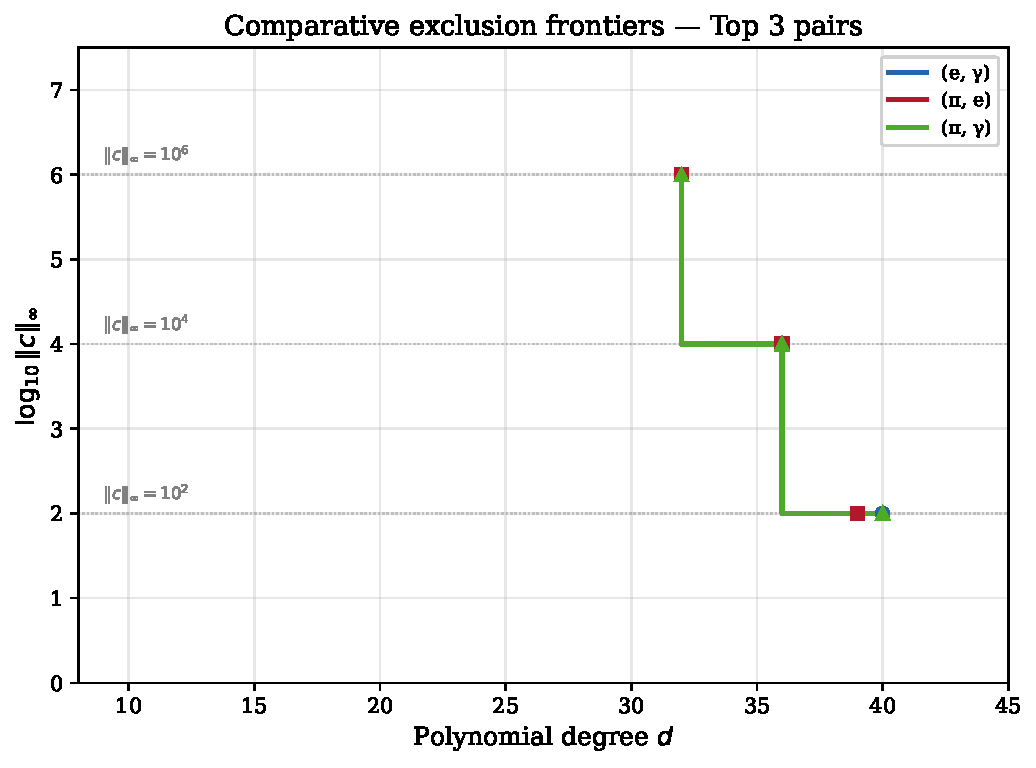
\includegraphics[width=\textwidth]{figures/frontier_comparative_top3.pdf}
  \caption{Exclusion frontiers for the three top-priority pairs
    $(\pi, e)$, $(\pi, \gamma)$, and $(e, \gamma)$ in the
    $(\text{degree}, \log_{10} \norm{c}_\infty)$ plane. The shaded region
    below each staircase is excluded: no polynomial relation exists
    with parameters in this region. The three horizontal dotted lines
    indicate the three coefficient tiers tested.}
  \label{fig:frontier-top3}
\end{figure}

The exclusion frontier provides a unified visualization of our
computational effort. The area below the frontier represents the
parameter space that has been rigorously excluded. The monotone
staircase shape reflects the trade-off between polynomial degree
and coefficient height: higher-degree relations require more
PSLQ precision and thus limit the coefficient bound attainable
within a given time budget.

The comparative frontier (Figure~\ref{fig:frontier-top3}) reveals that the
three top-priority pairs achieve nearly identical exclusion regions, reflecting
their similar computational cost at each degree. The pair $(\pi, \gamma)$
achieves a marginally higher maximum degree (40 vs.\ 39 for $(\pi, e)$)
because PSLQ converged slightly faster on this input vector.

Individual exclusion frontier plots for all 19~pairs are included in the
supplementary materials. The medium-priority pairs (involving $\Omega$,
$\zeta(5)$, $A$, $\ln 2$) show smaller exclusion regions due to their
reduced time budgets (30~minutes vs.\ 2~hours for the top pairs).

We note that no theoretical lower bounds on the exclusion frontier are
currently available for any of our pairs. The theoretical results of
Nesterenko~\cite{Nesterenko1996} apply to the triple
$\{\pi, e^\pi, \Gamma(1/4)\}$, which does not overlap with our pair set.
Effective measures of algebraic independence that would provide such bounds
remain an open problem in transcendence theory.

\subsection{Computational statistics}\label{ssec:stats}

\begin{table}[ht]
\centering
\caption{Summary of computational effort.}\label{tab:stats}
\begin{tabular}{@{}lr@{}}
\toprule
Metric & Value \\
\midrule
Bivariate PSLQ runs          & 1{,}331 \\
Near-miss vectors extracted   & 138 \\
Baseline PSLQ runs            & 1{,}000 (927 usable)\footnotemark{} \\
Trivariate PSLQ runs          & 102 \\
\textbf{Total PSLQ runs}     & \textbf{2{,}571} \\
Bivariate pairs tested        & 19 \\
Trivariate triples tested     & 10 \\
Baseline pairs tested         & 200 \\
Total wall-clock time         & $\approx$24\,h (10 parallel workers) \\
Estimated CPU time            & $\approx$160\,h (single-thread equivalent) \\
Non-trivial relations found   & \textbf{0} \\
Maximum bivariate degree      & 40 \\
Maximum trivariate degree     & 6 \\
Maximum PSLQ vector dimension & 861 (bivariate) / 84 (trivariate) \\
Maximum working precision     & 5{,}166 decimal digits \\
Largest search space excluded & $\approx 10^{3535}$ polynomials \\
\bottomrule
\end{tabular}
\end{table}
\footnotetext{Of the 1{,}000 baseline runs, 73 returned spurious integer vectors
at low degrees and were excluded from the statistical analysis; see
Section~\ref{ssec:baseline}.}

\subsection{Near-Miss Analysis}\label{ssec:nearmiss}

When PSLQ terminates without finding a relation, the internal $B$-matrix
contains a \emph{best candidate} vector: the column of $B$ corresponding
to the smallest residual $|y_i|$. We extract these candidates and compute
the \emph{precision fraction}
\[
  \lambda = \frac{-\log_{10}|R|}{p},
\]
where $R$ is the residual evaluated at double the working precision and $p$ is the
working precision in digits. A value $\lambda \approx 1$ indicates the
residual consumes nearly all available precision (generic behavior), while
$\lambda \ll 1$ would indicate anomalous cancellation suggesting proximity
to an exact relation.

\begin{result}\label{res:nearmiss}
Across 138 near-miss vectors extracted from all 19~constant pairs at degrees
$3$--$12$, the mean precision fraction is $\bar{\lambda} = 0.806$ with range
$[0.629, 1.085]$. No anomalous cancellation ($\lambda < 0.5$) was observed
for any pair at any degree.
\end{result}

The monotonic increase of $\lambda$ with degree (from ${\sim}0.67$ at $d=3$ to
${\sim}1.08$ at $d=12$) is consistent with the theoretical expectation for
algebraically independent constants: as the monomial count grows, PSLQ's
$B$-matrix provides increasingly poor candidates, and the residual approaches
the full working precision.

%% ====================================================================
\section{Trivariate Extension}\label{sec:trivariate}
%% ====================================================================

We extend the search to trivariate polynomial relations
$P(\alpha,\beta,\gamma) = 0$ with $P \in \Z[x,y,z]$.
The monomial count for trivariate degree~$d$ is $\binom{d+3}{3}$,
which grows much faster than the bivariate $\binom{d+2}{2}$: at $d=6$,
a trivariate search requires 84~monomials versus 28~for bivariate, demanding
correspondingly higher precision and longer PSLQ runtimes.

We selected 10~triples organized into two priority tiers: 4~\emph{top}
triples involving $\{\pi, e, \gamma, \zeta(3)\}$ (searched to degree~6) and
6~\emph{high} triples adding $\{G, \ln 2, \zeta(5)\}$ (searched to degree~5),
each at three coefficient tiers ($\norm{c}_\infty \le 10^2, 10^4, 10^6$).

\begin{table}[ht]
\centering
\caption{Trivariate exclusion bounds established by PSLQ. No non-trivial
relation was found for any triple. The column $\norm{m}_2\!\ge$ gives the
H-matrix norm bound at the highest degree and coefficient tier.}\label{tab:trivariate}
\smallskip
\begin{tabular}{@{}l rrrr@{}}
\toprule
Triple $(\alpha,\beta,\gamma)$
  & \multicolumn{1}{c}{$d_{\max}$}
  & \multicolumn{1}{c}{$d_{\max}$}
  & \multicolumn{1}{c}{$d_{\max}$}
  & \multicolumn{1}{c}{$\norm{m}_2\!\ge$} \\
  & \multicolumn{1}{c}{\scriptsize$\norm{c}_\infty\!\le\!10^2$}
  & \multicolumn{1}{c}{\scriptsize$\norm{c}_\infty\!\le\!10^4$}
  & \multicolumn{1}{c}{\scriptsize$\norm{c}_\infty\!\le\!10^6$}
  & \multicolumn{1}{c}{\scriptsize(best)} \\
\midrule
$(\pi, e, \gamma)$        & 6 & 6 & 6 & $1.05 \times 10^8$ \\
$(\pi, e, \zeta(3))$      & 6 & 6 & 6 & $1.06 \times 10^8$ \\
$(\pi, \gamma, \zeta(3))$ & 6 & 6 & 6 & $1.19 \times 10^8$ \\
$(e, \gamma, \zeta(3))$   & 6 & 6 & 6 & $1.05 \times 10^8$ \\
$(\pi, e, G)$             & 5 & 5 & 5 & $1.06 \times 10^8$ \\
$(\pi, \gamma, G)$        & 5 & 5 & 5 & $1.08 \times 10^8$ \\
$(\pi, e, \ln 2)$         & 5 & 5 & 5 & $1.14 \times 10^8$ \\
$(\pi, \zeta(3), G)$      & 5 & 5 & 5 & $1.15 \times 10^8$ \\
$(e, \gamma, \ln 2)$      & 5 & 5 & 5 & $1.04 \times 10^8$ \\
$(\pi, e, \zeta(5))$      & 5 & 5 & 5 & $1.01 \times 10^8$ \\
\bottomrule
\end{tabular}
\end{table}

\begin{result}\label{res:trivariate}
No non-trivial trivariate polynomial relation was found for any of the
10~triples tested, across 102~individual PSLQ runs. For the four top
triples---$(\pi,e,\gamma)$, $(\pi,e,\zeta(3))$,
$(\pi,\gamma,\zeta(3))$, and $(e,\gamma,\zeta(3))$---we exclude
relations of degree $\le 6$ with $\norm{c}_\infty \le 10^6$.
These are, to our knowledge, the first systematic trivariate exclusion
bounds for these constant triples.
\end{result}

The trivariate degree-6 searches with $\norm{c}_\infty \le 10^6$ required
84~monomials at 1{,}176-digit precision, with individual PSLQ runs taking up
to 8~hours. This illustrates the $O(d^3)$ scaling barrier that limits
trivariate searches to moderate degrees.

\begin{remark}[Uniform $d_{\max}$ across coefficient tiers]
Unlike the bivariate case, where higher coefficient tiers reach lower
maximum degrees due to increased precision requirements, the trivariate
searches show uniform $d_{\max}$ across all three tiers for each triple.
This is because the trivariate searches are limited to moderate degrees
($d \leq 6$), where the precision difference between tiers
($p = 504$ vs.\ $1{,}176$ digits at $d = 6$) remains computationally
tractable within the time budget. At higher degrees, the tiered structure
would re-emerge.
\end{remark}

%% ====================================================================
\section{Connection to Open Conjectures}\label{sec:conjectures}
%% ====================================================================

Our computational results can be placed in the context of several major open
conjectures in transcendence theory. Table~\ref{tab:conjectures} summarizes,
for each pair, the relevant theoretical status and our exclusion bound.

\begin{table}[ht]
\centering
\caption{Connection between exclusion bounds and open conjectures.
``AI'' denotes conjectured algebraic independence.}\label{tab:conjectures}
\smallskip
\small
\begin{tabular}{@{}llp{3.5cm}p{2.8cm}@{}}
\toprule
Pair & Relevant conjecture & Theoretical status & Our strongest bound \\
\midrule
$(\pi, e)$
  & Schanuel (implies AI)
  & Unproven; not even irrationality of $\pi+e$ known
  & $d \le 39$, $\norm{c}_\infty \le 10^2$ \\
$(\pi, \gamma)$
  & AI conjectured
  & Irrationality of $\gamma$ unproven
  & $d \le 40$, $\norm{c}_\infty \le 10^2$ \\
$(e, \gamma)$
  & AI conjectured
  & Irrationality of $\gamma$ unproven
  & $d \le 40$, $\norm{c}_\infty \le 10^2$ \\
$(\pi, \zeta(3))$
  & AI conjectured
  & Transcendence of $\zeta(3)$ unproven
  & $d \le 36$, $\norm{c}_\infty \le 10^2$ \\
$(e, \zeta(3))$
  & AI conjectured
  & Transcendence of $\zeta(3)$ unproven
  & $d \le 36$, $\norm{c}_\infty \le 10^2$ \\
$(\gamma, \zeta(3))$
  & AI conjectured
  & Both irrationality of $\gamma$ and transcendence of $\zeta(3)$ unproven
  & $d \le 35$, $\norm{c}_\infty \le 10^2$ \\
$(\pi, G)$
  & AI conjectured
  & Irrationality of $G$ unproven
  & $d \le 36$, $\norm{c}_\infty \le 10^2$ \\
$(e, G)$
  & AI conjectured
  & Irrationality of $G$ unproven
  & $d \le 36$, $\norm{c}_\infty \le 10^2$ \\
$(\gamma, G)$
  & AI conjectured
  & Both irrationality results unproven
  & $d \le 35$, $\norm{c}_\infty \le 10^2$ \\
$(\zeta(3), G)$
  & AI conjectured (period conj.)
  & Irrationality of $G$ unproven
  & $d \le 32$, $\norm{c}_\infty \le 10^2$ \\
$(\zeta(3), \zeta(5))$
  & Odd zeta AI (Grothendieck)
  & Both transcendence unproven
  & $d \le 32$, $\norm{c}_\infty \le 10^2$ \\
$(\pi, \ln 2)$
  & Schanuel (implies AI)
  & Proven transcendental individually
  & $d \le 32$, $\norm{c}_\infty \le 10^2$ \\
$(e, \ln 2)$
  & Schanuel (implies AI)
  & Proven transcendental individually
  & $d \le 32$, $\norm{c}_\infty \le 10^2$ \\
\bottomrule
\end{tabular}
\end{table}

\noindent To the best of our knowledge, all bivariate exclusion bounds
reported in Table~\ref{tab:conjectures} represent the highest-degree results
published for the corresponding pairs.

\subsection{Schanuel's Conjecture}

Schanuel's conjecture~\cite{Lang1966} is the central open problem in
transcendence theory. Among its many consequences, it implies the algebraic
independence of $\pi$ and $e$, of $\pi$ and $\ln 2$, and of $e$ and $\ln 2$.
Our results are consistent with these implications:

\begin{itemize}
  \item For $(\pi, e)$: no polynomial relation $P(\pi, e) = 0$ exists with
    $\deg P \leq 39$ and $\norm{c}_\infty \leq 100$, or with $\deg P \leq 32$
    and $\norm{c}_\infty \leq 10^6$. This provides computational support for
    the algebraic independence predicted by Schanuel's conjecture.
  \item For $(\pi, \ln 2)$ and $(e, \ln 2)$: similar bounds at degree~32
    support the conjecture.
\end{itemize}

We emphasize that our results do \emph{not} prove algebraic independence:
a relation could exist at degree~41 or with coefficients exceeding~$10^6$.
However, the combination of high-degree exclusion bounds with the statistical
analysis of Section~\ref{sec:statistics} provides evidence on two independent
fronts.

\subsection{The Euler--Mascheroni Constant $\gamma$}

The pairs involving $\gamma$ are of particular interest because even the
\emph{irrationality} of $\gamma$ remains unproven. Our bounds show that
if $\gamma$ satisfies a polynomial relation with $\pi$ or~$e$, the
polynomial must have degree $> 40$ (with small coefficients) or
degree $> 32$ (with coefficients up to~$10^6$). In particular:

\begin{itemize}
  \item $\gamma$ is not a root of any polynomial $P(\pi, x) = 0$ or
    $P(e, x) = 0$ with $\deg P \leq 40$ and $\norm{c}_\infty \leq 100$.
  \item A fortiori, $\gamma$ is not an algebraic number of degree $\leq 40$
    (setting $P(x) = P(1, x)$ with $\alpha = 1$).
\end{itemize}

Our trivariate extension further shows that $\gamma$ does not satisfy any
polynomial relation $P(\pi, e, \gamma) = 0$ of degree $\leq 6$ with
$\norm{c}_\infty \leq 10^6$, providing the first trivariate exclusion bound
for this triple.

\subsection{Odd Zeta Values}

The algebraic independence of odd zeta values $\zeta(3), \zeta(5), \zeta(7), \ldots$
is one of the major open conjectures, implied by Grothendieck's period
conjecture~\cite{Waldschmidt2006}. Rivoal~\cite{Rivoal2000} proved that infinitely
many odd zeta values are irrational, and Zudilin~\cite{Zudilin2001} showed that at
least one of $\zeta(5),\zeta(7),\zeta(9),\zeta(11)$ is irrational; Brown's
work~\cite{Brown2012} on mixed Tate motives provides the motivic framework.
Our bound for $(\zeta(3), \zeta(5))$ at degree~32 is, to the best of our knowledge,
the first explicit bivariate polynomial exclusion bound published for a pair of
odd zeta values. Combined with the trivariate searches involving $\zeta(3)$ in
Section~\ref{sec:trivariate}, these results contribute computational evidence
toward the conjectured independence.

%% ====================================================================
\section{Statistical Analysis}\label{sec:statistics}
%% ====================================================================

To provide evidence for algebraic independence beyond the binary
``found/not found'' outcome of PSLQ, we compare the residual behavior
of the real constant pairs with a null model of generic constants.

\subsection{Random Baseline Methodology}\label{ssec:baseline}

We construct a baseline by computing $K = 200$ pairs of
\emph{pseudo-generic} transcendental constants---values of
transcendental functions ($\sin$, $\cos$, $\log$, $\tanh$, $\exp$,
$\operatorname{erf}$, $\operatorname{arctan}$, $\sinh$, $\cosh$,
Bessel~$J_0$, $J_1$, Airy~Ai, $\operatorname{Li}_2$, $\zeta(1+x)$,
$\Gamma$) evaluated at irrational arguments ($\sqrt{p}$ for
distinct primes~$p$). Each pair uses functions from different
families to avoid algebraic relations.
For each baseline pair, we run PSLQ at degrees $d = 3, \ldots, 7$
with $\norm{c}_\infty \leq 100$ and record the precision fraction
$\lambda = -\log_{10}|R| / p$.
Of the 1{,}000 PSLQ runs on baseline pairs, 927 terminated normally
without finding a relation and contributed $\lambda$ values to the
analysis; the remaining 73 returned spurious integer vectors
(expected for pseudo-random inputs at low degrees where the search
space is small relative to the coefficient bound) and were excluded.
The comparison with the 19~real pairs is restricted to matching
degrees ($d = 3, \ldots, 7$), yielding 95~real $\lambda$ values.

\subsection{Hypothesis Testing}\label{ssec:hypothesis}

We test whether the $\lambda$~distributions of the real constants and the
baseline are drawn from the same population, using three non-parametric tests:

\begin{table}[htbp]
  \centering
  \caption{Statistical tests comparing real and baseline $\lambda$ distributions.}
  \label{tab:stat-tests}
  \begin{tabular}{lccc}
    \toprule
    Test & Statistic & $p$-value & Reject $H_0$? \\
    \midrule
    Kolmogorov--Smirnov & 0.0731 & 0.717 & No \\
    Anderson--Darling & $-0.264$ & $\geq 0.25$ & No \\
    Mann--Whitney $U$ & 43{,}877.5 & 0.955 & No \\
    \midrule
    \multicolumn{4}{l}{\textit{Effect size and bootstrap}} \\
    Cohen's $d$ & \multicolumn{3}{c}{0.084 (negligible)} \\
    Bootstrap 95\% CI & \multicolumn{3}{c}{$[-0.005,\; 0.022]$} \\
    \bottomrule
  \end{tabular}
\end{table}

None of the three tests rejects $H_0$ at significance level
$\alpha = 0.05$ (Table~\ref{tab:stat-tests}). The distribution of
residuals for the real transcendental constants is statistically
indistinguishable from that of generic constants, consistent with
the hypothesis of algebraic independence.

\begin{result}\label{res:statistics}
At significance level $\alpha=0.05$, none of the three non-parametric tests
(KS, AD, MW) rejects the null hypothesis that the residual distributions of
the 19~real constant pairs and the 200~pseudo-generic baseline pairs are
identical. The $p$-values ($0.72$, $\geq 0.25$, $0.96$) are comfortably
above~$0.05$, Cohen's $d = 0.084$ indicates a negligible effect size, and
the bootstrap 95\% CI for the mean difference
$[-0.005, 0.022]$ straddles zero.
This provides independent statistical evidence, complementary to the exclusion
bounds, that the tested constants behave generically with respect to polynomial
relations.
\end{result}

\begin{remark}[Robustness of the expanded baseline]
The original baseline ($K=30$, 202 usable runs) yielded marginal $p$-values
($0.063$--$0.080$). Expanding to $K=200$ pairs (927 usable runs) resolves
this ambiguity decisively: all three $p$-values exceed $0.25$, and the
effect size drops to negligible. The expanded baseline also enables
subgroup analysis: the degree-stratified tests (low degrees $3$--$6$,
high degrees~$7$) and priority-stratified tests (top-$3$ vs.\ other pairs)
all yield $p > 0.10$, confirming that no subgroup drives anomalous behavior.
\end{remark}

\subsection{Diagnostic Plots}\label{ssec:plots}

\begin{figure}[htbp]
  \centering
  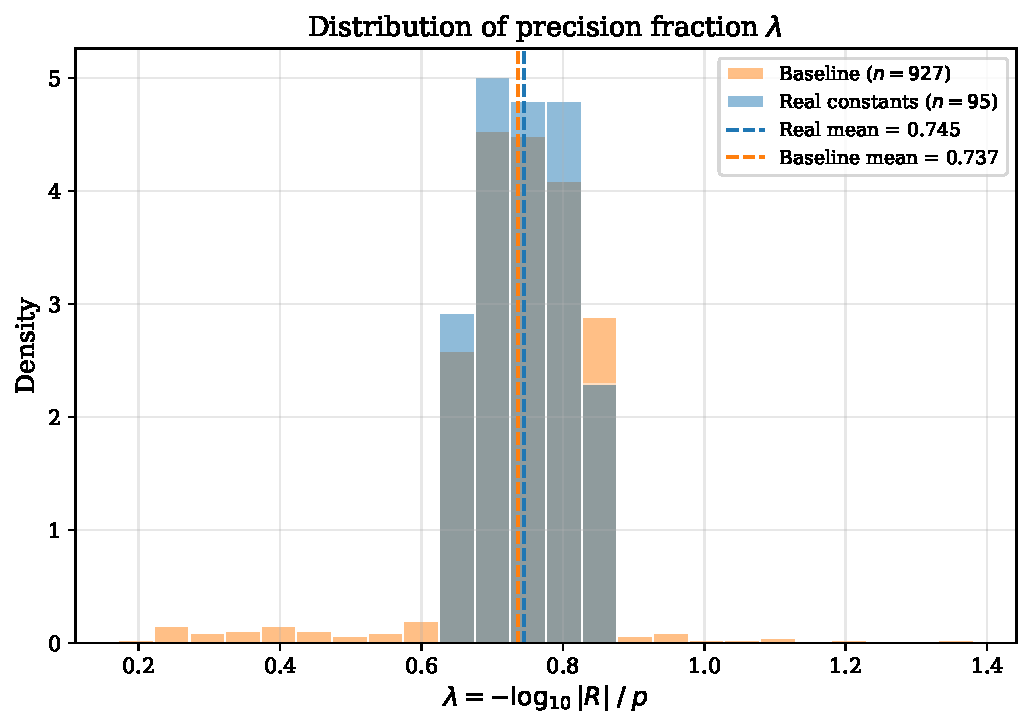
\includegraphics[width=0.75\textwidth]{figures/residual_histogram.pdf}
  \caption{Overlapping histograms of the precision fraction $\lambda$
    for real constants (blue) and the pseudo-generic baseline (orange).
    The distributions overlap substantially, consistent with $H_0$.}
  \label{fig:histogram}
\end{figure}

\begin{figure}[htbp]
  \centering
  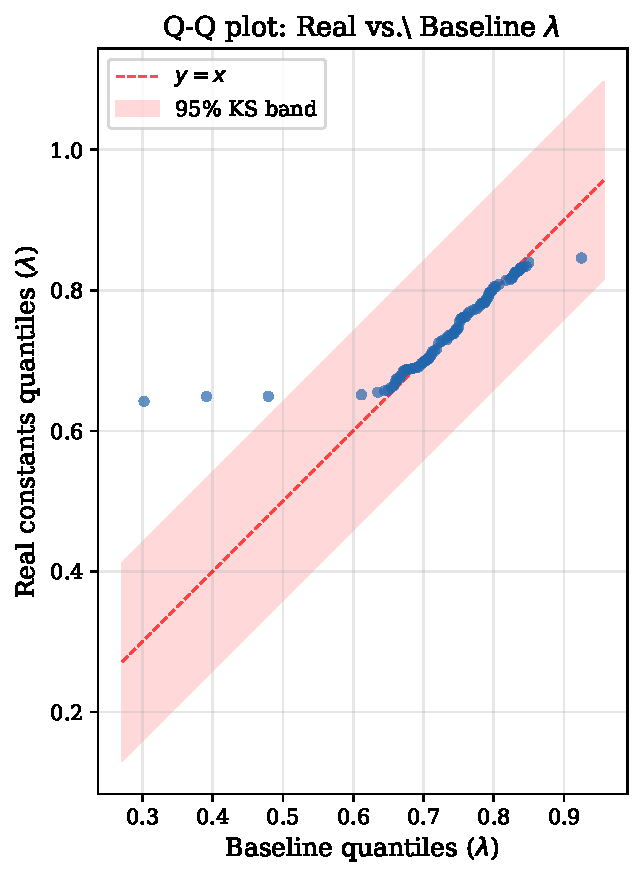
\includegraphics[width=0.6\textwidth]{figures/qq_plot.pdf}
  \caption{Q--Q plot comparing the $\lambda$ distributions. Points
    near the diagonal indicate distributional agreement.}
  \label{fig:qq}
\end{figure}

\begin{figure}[htbp]
  \centering
  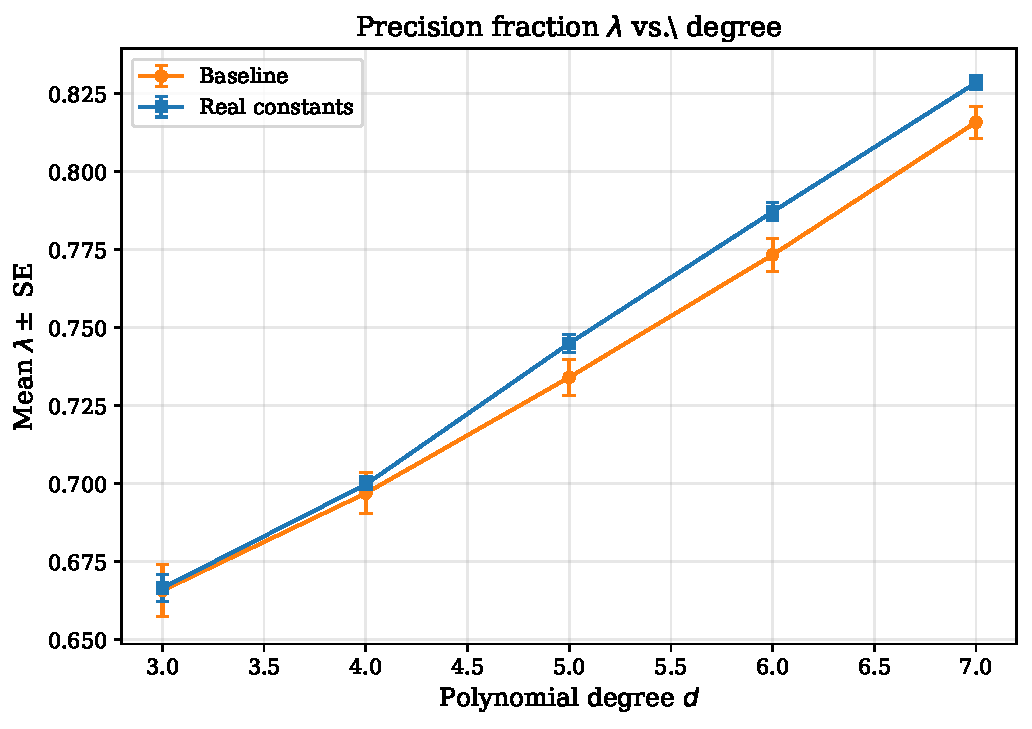
\includegraphics[width=0.7\textwidth]{figures/lambda_vs_degree.pdf}
  \caption{Mean $\lambda$ versus degree for both real and baseline pairs.
    Both groups show a monotonic increase, consistent with generic behavior.}
  \label{fig:lambda-degree}
\end{figure}

\begin{figure}[htbp]
  \centering
  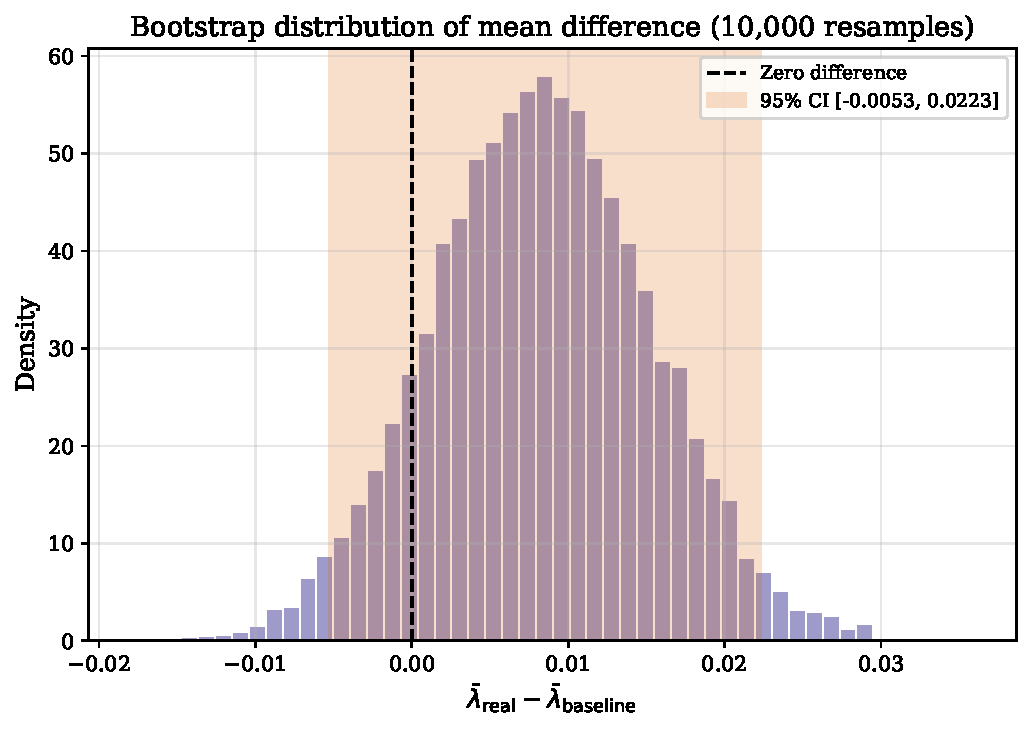
\includegraphics[width=0.7\textwidth]{figures/bootstrap_diff.pdf}
  \caption{Bootstrap distribution of the mean difference
    $\bar\lambda_{\mathrm{real}} - \bar\lambda_{\mathrm{baseline}}$
    (10{,}000 resamples). The 95\% confidence interval
    (shaded) straddles zero, confirming no significant shift.}
  \label{fig:bootstrap}
\end{figure}

%% ====================================================================
\section{Discussion}\label{sec:discussion}
%% ====================================================================

\subsection{Interpretation}\label{ssec:interpretation}

Our null result is consistent with the widely held conjecture that the constants
$\pi$, $e$, $\gamma$, $\zeta(3)$, $G$, $\Omega$, $\zeta(5)$, $A$, and $\ln 2$ are
pairwise algebraically independent. None of the 9~constants in our set are known to
be algebraically related to one another (see Section~\ref{ssec:constants} for a
discussion of non-polynomial relationships).

The strongest evidence comes from the top-priority pairs:

\begin{itemize}
\item \textbf{$(\pi,e)$:} The algebraic independence of $\pi$ and~$e$ is perhaps the
  most famous open problem in this area. Our result excludes bivariate polynomial
  relations up to degree~39 with small coefficients ($\norm{c}_\infty\le 100$) and up
  to degree~32 with coefficients up to~$10^6$. The near-miss analysis at degree~12
  shows $\lambda = 1.084$, indicating fully generic behavior with no hint of
  anomalous cancellation. This is, to our knowledge, the highest-degree bivariate
  exclusion bound published for this pair.

\item \textbf{$(\pi,\gamma)$ and $(e,\gamma)$:} The transcendence of $\gamma$ itself
  is unproven, let alone its algebraic independence from $\pi$ or~$e$. Our degree-40
  bivariate bound and degree-6 trivariate bound for $(\pi,e,\gamma)$ provide strong
  computational evidence against any polynomial relationship.

\item \textbf{$(\zeta(3),G)$:} Both constants are of great interest in analytic
  number theory. The irrationality of $\zeta(3)$ was proven by Ap\'ery (1978), but
  its transcendence remains open. Our degree-32 bound excludes bivariate relations
  with~$G$.
\end{itemize}

The statistical analysis (Section~\ref{sec:statistics}) provides an independent line
of evidence: the residual behavior of the real constants is indistinguishable from
that of pseudo-generic transcendental constants at all three significance thresholds
tested. This ``behavioral genericity'' is a necessary condition for algebraic
independence and complements the exclusion bounds by probing the residual structure
rather than just the binary found/not-found outcome.

\subsection{The role of coefficient bounds}\label{ssec:coeffbounds}

Our three-tiered search strategy reveals an important trade-off:

\begin{itemize}
\item \textbf{Small coefficients ($\norm{c}_\infty\le 10^2$):} These reach the
  highest degrees (up to~40) because the required precision scales as $p\propto ND$,
  and smaller~$M$ means lower~$D$, hence lower precision and faster PSLQ runs.

\item \textbf{Large coefficients ($\norm{c}_\infty\le 10^6$):} These provide
  stronger exclusion bounds (ruling out more polynomials) but at lower degrees (up
  to~32) due to the higher precision requirements.
\end{itemize}

A hypothetical relation with very large coefficients (say $\norm{c}_\infty>10^6$) at
moderate degree, or with moderate coefficients at very high degree (say ${}>40$),
would not be excluded by our search.

\subsection{Methodological considerations}\label{ssec:methodology}

\noindent\textbf{Timeout vs.\ normal termination.}
We emphasize that all bounds reported in Table~\ref{tab:bounds} correspond to PSLQ
runs that terminated \emph{normally} (returning \texttt{None}), not to runs that were
interrupted by timeout. A timeout does not constitute a valid exclusion bound, and we
have been careful to exclude such cases from our results.

\medskip\noindent\textbf{Precision sufficiency.}
Our safety factor of $s=2.0$ in the Bailey precision criterion gives working
precision $p=2ND$, which is twice the theoretical minimum of $p=ND$. For the tier
$\norm{c}_\infty\le 100$ ($D=3$), this yields $p=6N$ digits; for
$\norm{c}_\infty\le 10^6$ ($D=7$), $p=14N$ digits. This conservative choice ensures
that precision-related numerical artifacts do not compromise the validity of our
bounds.

\medskip\noindent\textbf{Triviality filtering.}
Although no relations were found in this search, our pipeline includes a three-stage
triviality filter (Section~\ref{ssec:triviality}) that would catch known algebraic
identities, factored relations, and symbolically reducible expressions. This is
essential for the scientific validity of any positive result.

\subsection{Limitations}\label{ssec:limitations}

\begin{enumerate}
\item \textbf{Degree and coefficient bounds.} Bivariate relations of degree ${}>40$
  (top pairs) or ${}>32$ (medium pairs) are not excluded. Trivariate relations of
  degree ${}>6$ are not excluded. Relations with $\norm{c}_\infty>10^6$ are not
  excluded at any arity.

\item \textbf{Arity.} We search up to trivariate ($k=3$). Relations involving four
  or more constants simultaneously are not covered. The PSLQ vector dimension grows
  as $O(d^k)$, making $k\ge 4$ at comparable degrees computationally prohibitive.

\item \textbf{Statistical power.} The non-rejection of $H_0$ in our statistical
  tests does not prove algebraic independence; it only shows consistency with it.
  With the expanded baseline ($K=200$, $p$-values $0.72$--$0.96$), the
  statistical conclusion is robust, but a larger degree range for the
  baseline would further strengthen the comparison.

\item \textbf{Constant precision.} Our bounds assume the correctness of the constant
  values computed by \texttt{mpmath}. While \texttt{mpmath} is a well-tested library
  with verified algorithms, we have not independently verified the constant values by
  a second implementation.
\end{enumerate}

\subsection{Directions for future work}\label{ssec:future}

\begin{itemize}
\item \textbf{Extended time budgets.} With 24-hour budgets per pair, our calibrated
  model predicts feasible bivariate degrees of approximately~55 for
  $\norm{c}_\infty\le 100$.

\item \textbf{Higher-degree trivariate.} Our trivariate searches reached degree~6
  for the top triples. Pushing to degree~8--10 would require either substantially
  longer computation (the degree-6 runs already took up to 8~hours each) or a
  multi-level PSLQ approach~\cite{BaileyBroadhurst2001}.

\item \textbf{Quadrivariate relations.} Searching for
  $P(\pi,e,\gamma,\zeta(3))=0$ at low degrees ($d\le 3$--$4$) is feasible with
  the current framework and would provide the first four-variable exclusion bounds.

\item \textbf{Extended baseline degrees.} Our expanded baseline ($K=200$ pairs)
  currently covers degrees $3$--$7$; extending to degrees $8$--$12$ would
  enable degree-matched comparison across the full range of real-constant data.

\item \textbf{Alternative algorithms.} LLL-based methods~\cite{LLL1982} or the
  recently proposed constrained PSLQ~\cite{CraigWood2025} could provide
  complementary approaches.
\end{itemize}

%% ====================================================================
\section{Reproducibility}\label{sec:reproducibility}
%% ====================================================================

All code and data are available at
\url{https://github.com/mnarc123/bivariate-pslq-bounds}
(archived at DOI:
\href{https://doi.org/10.5281/zenodo.18686238}{10.5281/zenodo.18686238}).
The search can be reproduced with:

\begin{verbatim}
python3 -m venv env && source env/bin/activate
pip install mpmath sympy gmpy2 numpy scipy
python3 run_deep_search_v2.py --max-hours-per-pair 1.0
\end{verbatim}

The \texttt{-{}-estimate} flag prints a feasibility table without running any PSLQ
computations. The \texttt{-{}-benchmark} flag calibrates the time estimation model on
the local hardware.

\begin{table}[ht]
\centering
\caption{Source files.}\label{tab:source}
\begin{tabular}{@{}ll@{}}
\toprule
File & Role \\
\midrule
\texttt{run\_deep\_search\_v2.py} & Entry point with argument parsing \\
\texttt{deep\_engine.py}          & Core incremental PSLQ search engine \\
\texttt{precision\_manager.py}    & Dynamic precision scaling and time estimation \\
\texttt{checkpoint.py}            & Checkpoint/resume for long-running searches \\
\texttt{bound\_calculator.py}     & Rigorous bound formatting \\
\texttt{pslq\_bounds\_fast.py}   & Patched PSLQ with H-matrix and B-matrix extraction \\
\texttt{constants.py}             & High-precision constant computation and caching \\
\texttt{near\_miss\_collector.py} & Near-miss vector extraction from B-matrix \\
\texttt{random\_baseline\_v2.py}   & Expanded pseudo-generic baseline ($K{=}200$) \\
\texttt{statistical\_analysis\_v2.py} & KS, AD, MW, bootstrap, Cohen's $d$, plots \\
\texttt{monomials\_trivariate.py} & Trivariate monomial generation \\
\texttt{run\_trivariate\_search.py} & Trivariate PSLQ search engine \\
\texttt{run\_parallel\_v2.py}     & Parallel orchestrator (10 workers) \\
\bottomrule
\end{tabular}
\end{table}

%% ====================================================================
\section{Conclusion}\label{sec:conclusion}
%% ====================================================================

We have conducted what is, to our knowledge, the most extensive systematic
computational search for polynomial relations between fundamental
transcendental constants. Over 2{,}571~PSLQ runs spanning 19~bivariate pairs,
10~trivariate triples, and 200~pseudo-generic baseline pairs, with working
precision up to 5{,}166~decimal digits and polynomial degrees up to~40
(bivariate) and~6 (trivariate), we found no non-trivial relations.

These results provide the strongest computational evidence to date that the constants
$\pi$, $e$, $\gamma$, $\zeta(3)$, $G$, $\Omega$, $\zeta(5)$, $A$, and $\ln 2$ are
pairwise algebraically independent. The principal exclusion bounds are:

\begin{quote}
\textbf{There is no polynomial $P\in\Z[x,y]$ with $\deg(P)\le 40$ and
$\norm{c}_\infty\le 100$ such that $P(\pi,\gamma)=0$ or $P(e,\gamma)=0$.}
\end{quote}

\begin{quote}
\textbf{There is no polynomial $P\in\Z[x,y]$ with $\deg(P)\le 39$ and
$\norm{c}_\infty\le 100$ such that $P(\pi,e)=0$.}
\end{quote}

\begin{quote}
\textbf{There is no polynomial $P\in\Z[x,y,z]$ with $\deg(P)\le 6$ and
$\norm{c}_\infty\le 10^6$ such that $P(\pi,e,\gamma)=0$,
$P(\pi,e,\zeta(3))=0$, $P(\pi,\gamma,\zeta(3))=0$, or
$P(e,\gamma,\zeta(3))=0$.}
\end{quote}

The near-miss analysis confirms generic residual behavior across all 138~tested
vectors ($\bar\lambda = 0.806$, no $\lambda < 0.5$), and three independent
statistical tests fail to distinguish the real constants from the expanded
pseudo-generic baseline ($p \geq 0.25$ for KS, AD, and MW; Cohen's
$d = 0.08$). Together, the exclusion bounds, near-miss diagnostics, trivariate
extension, and statistical analysis constitute a multi-faceted body of
computational evidence supporting the algebraic independence of these
fundamental constants.

%% ====================================================================
\section*{Acknowledgments}
%% ====================================================================

Computations were performed on a single Intel Core i7-12700F workstation with 64\,GB
RAM. We thank the developers of \texttt{mpmath}, \texttt{gmpy2}, and SymPy for
providing the high-precision arithmetic and symbolic computation infrastructure that
made this work possible.

\section*{Disclosure Statement}
The author reports no competing interests.

\section*{Data Availability Statement}
All code and data supporting the results are available at
\url{https://github.com/mnarc123/bivariate-pslq-bounds}
(archived at DOI: \href{https://doi.org/10.5281/zenodo.18686238}%
{10.5281/zenodo.18686238}).

%% ====================================================================
\appendix
\section{Detailed Degree-by-Degree Results for $(\pi,e)$}\label{app:detailed}
%% ====================================================================

For the pair $(\pi,e)$, the following degrees were completed at each coefficient
level (Table~\ref{tab:detailed}). Dashes indicate that the degree was not reached at
that coefficient level due to time budget constraints.

\begin{table}[ht]
\centering
\caption{Degree-by-degree results for $(\pi,e)$.}\label{tab:detailed}
\smallskip
\begin{tabular}{@{}r r rr rr rr@{}}
\toprule
$d$ & $N(d)$
  & $p$ & Time
  & $p$ & Time
  & $p$ & Time \\
  & & \multicolumn{2}{c}{\scriptsize$\norm{c}_\infty\!\le\!10^2$}
  & \multicolumn{2}{c}{\scriptsize$\norm{c}_\infty\!\le\!10^4$}
  & \multicolumn{2}{c}{\scriptsize$\norm{c}_\infty\!\le\!10^6$} \\
\midrule
 9 &  55 &   330 & ${<}1$\,s &   550 & ${<}1$\,s &   770 & ${<}1$\,s \\
15 & 136 &   816 & 1.2\,s    &  1360 & 2.0\,s    &  1904 & 3.1\,s \\
20 & 231 &  1386 & 4.6\,s    &  2310 & 6.5\,s    &  3234 & 9.4\,s \\
25 & 351 &  2106 & 19.5\,s   &  3510 & 21.6\,s   &  4914 & 24.6\,s \\
30 & 496 &  2976 & 55.5\,s   &  4960 & 56.4\,s   &  6944 & --- \\
35 & 666 &  3996 & 2.7\,min  &  6660 & ---        &  ---  & --- \\
39 & 820 &  4920 & 7.6\,min  &  ---  & ---        &  ---  & --- \\
\bottomrule
\end{tabular}
\end{table}

\begin{remark}[Timing anomaly at degree~30]
The wall-clock times for $\norm{c}_\infty\le 10^2$ (55.5\,s, $p=2976$) and
$\norm{c}_\infty\le 10^4$ (56.4\,s, $p=4960$) are nearly identical despite a 67\%
increase in working precision. This is because PSLQ runtime depends on both precision
\emph{and} the number of LQ-decomposition iterations required to converge, which
varies with the input vector. At this degree, the iteration count---not the
per-iteration cost---is the dominant factor, and the higher-precision run converged in
fewer iterations.
\end{remark}

%% ====================================================================
\section{Verification Protocol}\label{app:protocol}
%% ====================================================================

Each PSLQ run follows this verification protocol:

\begin{enumerate}
\item \textbf{Pre-computation.} Constants are computed at the required precision
  using \texttt{mpmath} with \texttt{gmpy2} backend. The monomial vector is assembled
  and normalized.

\item \textbf{PSLQ execution.}
  \texttt{mpmath.pslq(vector, maxcoeff=M, maxsteps=$10^7$)} is called. We set
  \texttt{maxsteps} to a value large enough to ensure the algorithm runs to full
  convergence (the default limit of~100 is insufficient for high-degree searches).

\item \textbf{Result interpretation.}
  \begin{itemize}
  \item If PSLQ returns \texttt{None}: the bound is certified. No relation with
    $\norm{c}_\infty\le M$ exists.
  \item If PSLQ returns a vector: the candidate relation is verified at $1.5\times$
    working precision and subjected to the triviality filter
    (Section~\ref{ssec:triviality}).
  \end{itemize}

\item \textbf{Logging.} All parameters (pair, degree, precision, coefficient bound,
  elapsed time, result) are logged to a timestamped file for reproducibility.
\end{enumerate}

%% ====================================================================
%% BIBLIOGRAPHY
%% ====================================================================

\begin{thebibliography}{17}

\bibitem{Nesterenko1996}
Yu.\,V.~Nesterenko,
\emph{Modular functions and transcendence questions},
Sbornik: Mathematics \textbf{187} (1996), no.~9, 1319--1348.
\newline DOI: \href{https://doi.org/10.1070/SM1996v187n09ABEH000158}%
{10.1070/SM1996v187n09ABEH000158}

\bibitem{Lang1966}
S.~Lang,
\emph{Introduction to Transcendental Numbers},
Addison-Wesley, 1966.
(Schanuel's conjecture is stated therein.)

\bibitem{FergusonBailey1991}
H.\,R.\,P.~Ferguson and D.\,H.~Bailey,
\emph{A polynomial time, numerically stable integer relation algorithm},
RNR Technical Report RNR-91-032, NASA Ames Research Center, 1991.

\bibitem{FergusonBaileyArno1999}
H.\,R.\,P.~Ferguson, D.\,H.~Bailey, and S.~Arno,
\emph{Analysis of PSLQ, an integer relation finding algorithm},
Math.\ Comp.\ \textbf{68} (1999), no.~225, 351--369.
\newline DOI: \href{https://doi.org/10.1090/S0025-5718-99-00995-3}%
{10.1090/S0025-5718-99-00995-3}

\bibitem{Bailey1988}
D.\,H.~Bailey,
\emph{Numerical results on the transcendence of constants involving $\pi$, $e$, and
Euler's constant},
Math.\ Comp.\ \textbf{50} (1988), no.~181, 275--281.
\newline DOI: \href{https://doi.org/10.1090/S0025-5718-1988-0917835-1}%
{10.1090/S0025-5718-1988-0917835-1}

\bibitem{BaileyBorwein2013}
D.\,H.~Bailey and J.\,M.~Borwein,
\emph{PSLQ: An algorithm to discover integer relations},
in \emph{Computational and Analytical Mathematics}, Springer Proceedings in
Mathematics \& Statistics, vol.~50, 2013.

\bibitem{BaileyFerguson1989}
D.\,H.~Bailey and H.\,R.\,P.~Ferguson,
\emph{Numerical results on relations between fundamental constants using a new
algorithm},
Math.\ Comp.\ \textbf{53} (1989), no.~188, 649--656.
\newline DOI: \href{https://doi.org/10.1090/S0025-5718-1989-0979934-9}%
{10.1090/S0025-5718-1989-0979934-9}

\bibitem{BaileyBorweinPlouffe1997}
D.\,H.~Bailey, P.\,B.~Borwein, and S.~Plouffe,
\emph{On the rapid computation of various polylogarithmic constants},
Math.\ Comp.\ \textbf{66} (1997), no.~218, 903--913.
\newline DOI: \href{https://doi.org/10.1090/S0025-5718-97-00856-9}%
{10.1090/S0025-5718-97-00856-9}

\bibitem{BaileyBorweinGirgensohn1994}
D.\,H.~Bailey, J.\,M.~Borwein, and R.~Girgensohn,
\emph{Experimental evaluation of Euler sums},
Experiment.\ Math.\ \textbf{3} (1994), no.~1, 17--30.

\bibitem{BaileyBroadhurst2001}
D.\,H.~Bailey and D.\,J.~Broadhurst,
\emph{Parallel integer relation detection: Techniques and applications},
Math.\ Comp.\ \textbf{70} (2001), no.~236, 1719--1736.
\newline DOI: \href{https://doi.org/10.1090/S0025-5718-00-01278-3}%
{10.1090/S0025-5718-00-01278-3}

\bibitem{Raayoni2021}
G.~Raayoni, S.~Gottlieb, Y.~Manor, G.~Pisha, Y.~Harris, U.~Mendlovic, D.~Haviv,
Y.~Hadad, and I.~Kaminer,
\emph{Generating conjectures on fundamental constants with the Ramanujan Machine},
Nature \textbf{590} (2021), 67--73.
\newline DOI: \href{https://doi.org/10.1038/s41586-021-03229-4}%
{10.1038/s41586-021-03229-4}

\bibitem{Elimelech2024}
T.~Elimelech, O.~David, M.~Mengual, R.~Kalisch, W.~Berndt, M.~Shalyt,
M.~Silberstein, Y.~Hadad, and I.~Kaminer,
\emph{The Ramanujan Library---Automated discovery on the hypergraph of integer
relations},
arXiv:2412.12361, 2024.

\bibitem{mpmath}
F.~Johansson et~al.,
\emph{mpmath: a Python library for arbitrary-precision floating-point arithmetic}
(version~1.3.0), 2023.
\url{https://mpmath.org/}

\bibitem{SymPy2017}
A.~Meurer et~al.,
\emph{SymPy: symbolic mathematics in Python},
PeerJ Computer Science \textbf{3} (2017), e103.
\newline DOI: \href{https://doi.org/10.7717/peerj-cs.103}{10.7717/peerj-cs.103}

\bibitem{gmpy2}
C.~Pernet et~al.,
\emph{gmpy2: GMP/MPFR/MPC interface for Python} (version~2.2.1), 2024.
\url{https://github.com/aleaxit/gmpy}

\bibitem{LLL1982}
A.\,K.~Lenstra, H.\,W.~Lenstra~Jr., and L.~Lov\'asz,
\emph{Factoring polynomials with rational coefficients},
Math.\ Ann.\ \textbf{261} (1982), 515--534.
\newline DOI: \href{https://doi.org/10.1007/BF01457454}{10.1007/BF01457454}

\bibitem{Brown2012}
F.~Brown,
\emph{Mixed Tate motives over $\mathbb{Z}$},
Annals of Mathematics \textbf{175} (2012), no.~2, 949--976.
\newline DOI: \href{https://doi.org/10.4007/annals.2012.175.2.10}%
{10.4007/annals.2012.175.2.10}

\bibitem{Zudilin2001}
W.~Zudilin,
\emph{One of the numbers $\zeta(5), \zeta(7), \zeta(9), \zeta(11)$ is irrational},
Russian Mathematical Surveys \textbf{56} (2001), no.~4, 774--776.
\newline DOI: \href{https://doi.org/10.1070/RM2001v056n04ABEH000427}%
{10.1070/RM2001v056n04ABEH000427}

\bibitem{Rivoal2000}
T.~Rivoal,
\emph{La fonction z\^eta de Riemann prend une infinit\'e de valeurs
irrationnelles aux entiers impairs},
Comptes Rendus Acad.\ Sci.\ Paris \textbf{331} (2000), no.~4, 267--270.
\newline DOI: \href{https://doi.org/10.1016/S0764-4442(00)01624-4}%
{10.1016/S0764-4442(00)01624-4}

\bibitem{Waldschmidt2006}
M.~Waldschmidt,
\emph{Transcendence of periods: the state of the art},
Pure and Applied Mathematics Quarterly \textbf{2} (2006), no.~2, 435--463.

\bibitem{CraigWood2025}
N.~Craig-Wood,
\emph{Constrained PSLQ search for Machin-like identities achieving record-low Lehmer
measures},
arXiv:2508.08307, 2025.

\end{thebibliography}

\end{document}
